% ============================================================================
\section{End-to-end ASR}
% ============================================================================

% --- Stanford CS224S lec10, slides 24--30, 32: Connectionist Temporal Classification ---
\begin{frame}{Connectionist Temporal Classification (CTC)}
  \textbf{End-to-end alternative to hybrid HMM--DNN:} map audio directly to transcript tokens (characters, phonemes, BPE).
\end{frame}

\begin{frame}{HMM-free recognition with CTC}
  \begin{itemize}
    \item DNN approximates $P(a \mid x)$ over output tokens; no separate HMM state topology for alignment.
  \end{itemize}
  \centering
  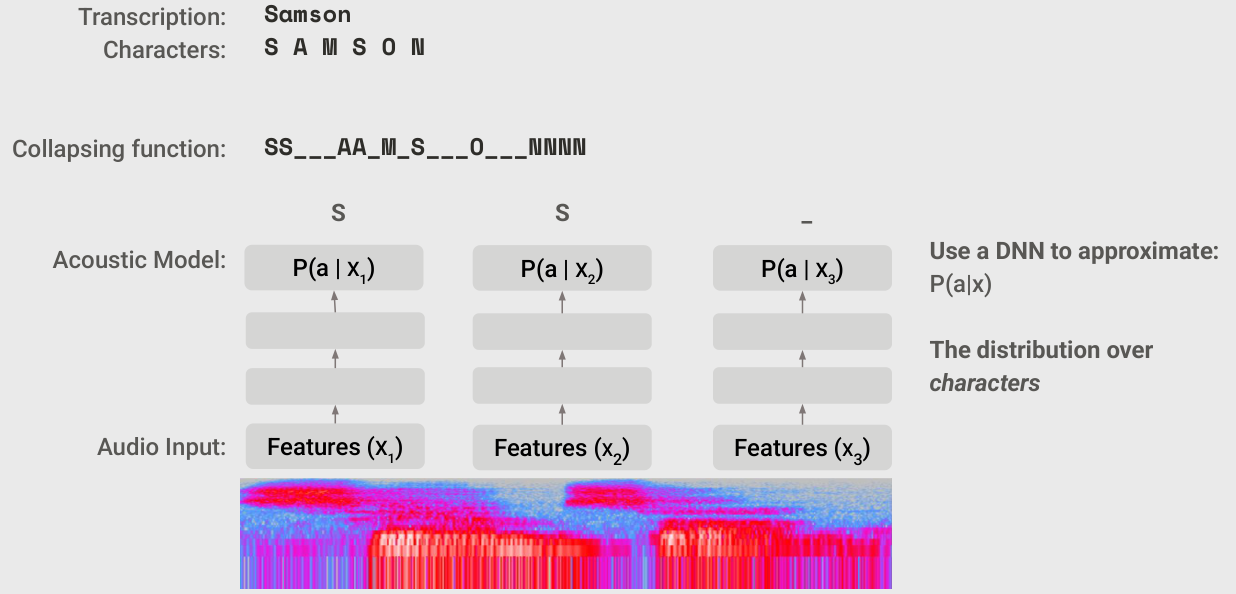
\includegraphics[width=\textwidth,height=0.78\textheight,keepaspectratio]{assets/New-Lecture-STT/cs224s_lec10_slide_25.png}
\end{frame}

\begin{frame}{CTC output assumptions}
  \textbf{CTC output assumptions}

  \begin{itemize}\footnotesize
    \item Each timestep $t$ the model outputs $P(a \mid X_{1:T})$, which can either be an output token (character, phoneme) or ``blank''.
    \item \emph{Assume:} Input sequence (length $T$) $\geq$ output sequence length (safe assumption in ASR).
    \item \textbf{Collapsing rule:} Ignore all blank tokens, and ignore repeated outputs of the same token.
  \end{itemize}
  \centering
  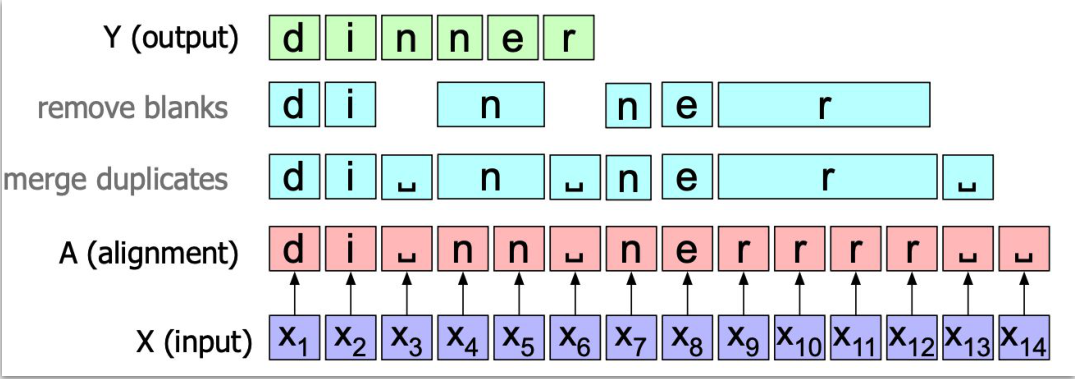
\includegraphics[width=\textwidth,height=0.78\textheight,keepaspectratio]{assets/New-Lecture-STT/cs224s_lec10_slide_26.png}
\end{frame}

\begin{frame}{CTC collapsing. Sum over all possible alignments}
  \centering
  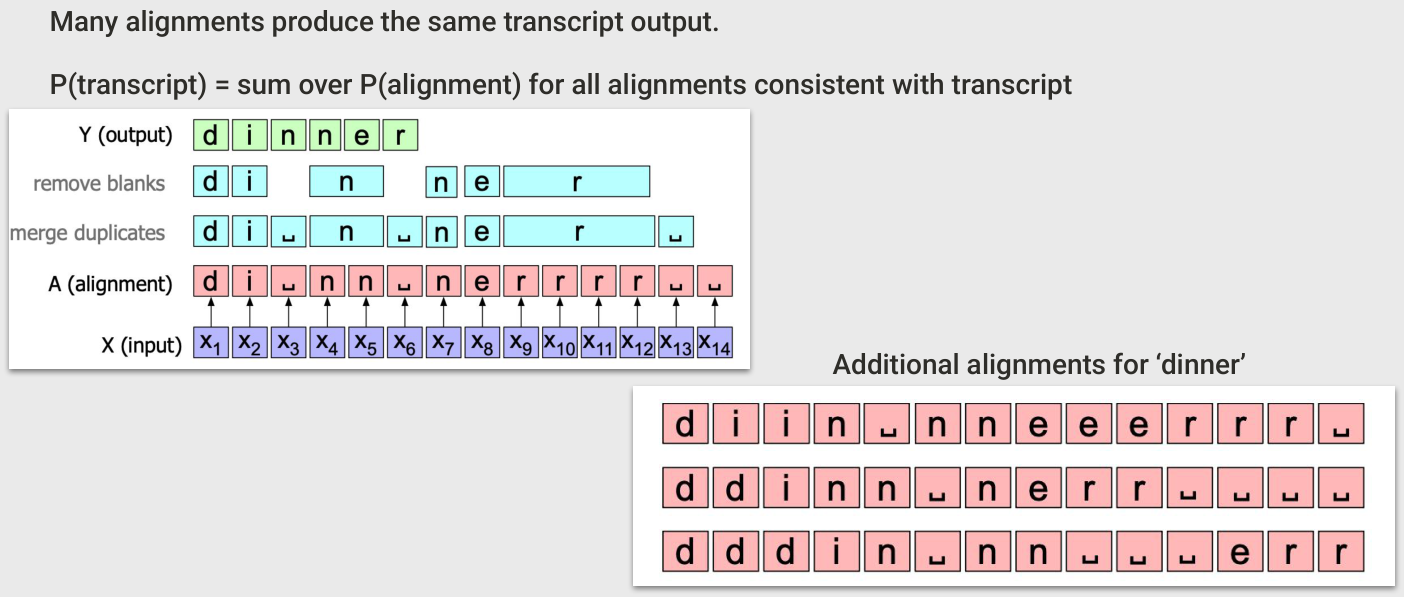
\includegraphics[width=\textwidth,height=0.78\textheight,keepaspectratio]{assets/New-Lecture-STT/cs224s_lec10_slide_27.png}
\end{frame}

\begin{frame}{Real example. Full utterance with blank token}
  \centering
  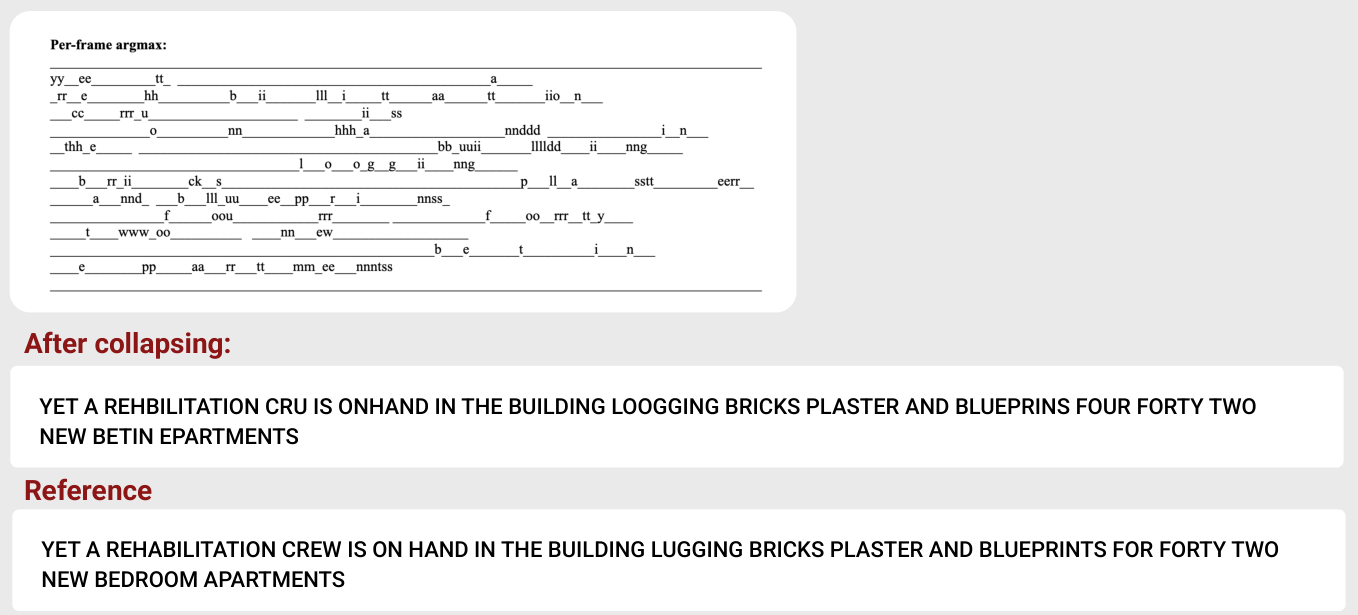
\includegraphics[width=\textwidth,height=0.82\textheight,keepaspectratio]{assets/New-Lecture-STT/cs224s_lec10_slide_28.png}
\end{frame}

\begin{frame}{Example CTC results. No word lexicon or LM (WSJ corpus)}
  \centering
  
\includegraphics[width=\textwidth,height=0.82\textheight,keepaspectratio]{assets/New-Lecture-STT/cs224s_lec10_slide_29.png}
\end{frame}

\begin{frame}{CTC loss function}
  \begin{itemize}\footnotesize
    \item Labels at each time index are \textbf{conditionally independent} given the audio input (like HMMs):
      \[
        \Pr(a \mid x) = \prod_{t=1}^T \Pr(a_t \mid x)
      \]
    \item \textbf{CTC loss:} Negative log probability of the target transcription $y^*$, summed over all possible time-level labelings $a$ that collapse to $y^*$:
      \[
        \text{CTC}(x) = -\log \Pr(y^*|x), \qquad
        \Pr(y|x) = \sum_{a \in B^{-1}(y)} \Pr(a|x)
      \]
    \item For sequence length $T=3$, transcript $HI$:
      \begin{itemize}
        \item All possible pre-collapsed/time-level labelings: \texttt{HI}, \texttt{H\_I}, \texttt{\_HI}, \texttt{HHI}, \texttt{H\_II}
      \end{itemize}
    \item The final loss maximizes the probability of the transcript $y^*$.
    \item \textbf{Insights:} Conditional independence allows us to compute outputs for each $t$ in parallel.
      \begin{itemize}
        \item Blank + collapsing enables efficient, exact summation over all alignments.
      \end{itemize}
  \end{itemize}
\end{frame}

\begin{frame}{CTC inference: Most likely alignment}
  \begin{columns}[T]
    \begin{column}{0.50\textwidth}
      \begin{itemize}
        \item \textbf{Output model assumes conditional independence.}
        \item Each $t$ most likely output depends only on inputs (not auto-regressive).
        \item Most likely pre-collapsed output is simply the sequence of argmax outputs for each $t$.
        \item Run CTC collapsing to obtain transcript.
      \end{itemize}
    \end{column}
    \begin{column}{0.48\textwidth}
      \centering
      % Placeholder for image
      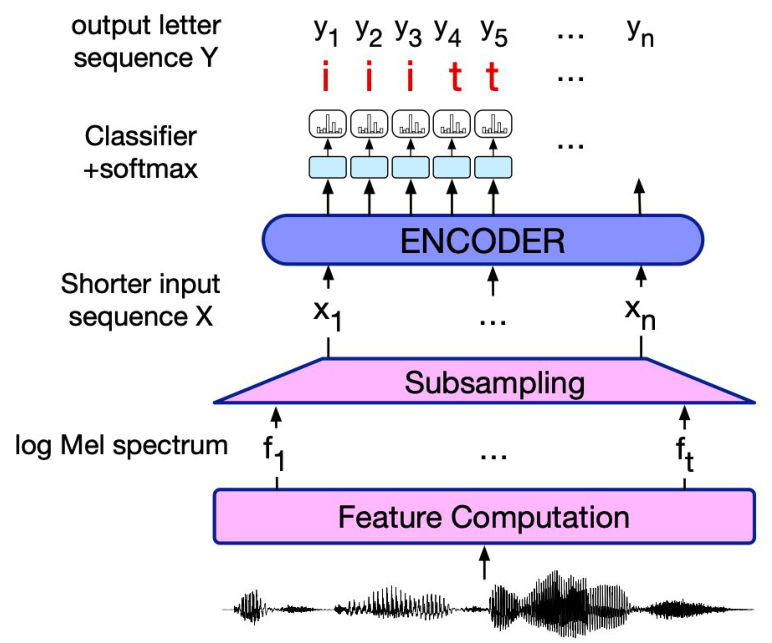
\includegraphics[width=\textwidth,keepaspectratio]{assets/New-Lecture-STT/cs224s_lec10_slide_32.png}
    \end{column}
  \end{columns}
\end{frame}

% --- Stanford CS224S lec10, slide 47 ---
\begin{frame}{Improving on CTC: RNN-Transducer (RNN-T) output model}
  \begin{itemize}\footnotesize
    \item Add network that reasons over sequence of non-blank characters/tokens and input sequence
    \item Decoding outputs each transcript token only once. Optional blanks between. Variation on CTC
    \item Prediction network often pre-trained with CTC. Encoder provides transformed features for each $t$
  \end{itemize}
  \centering
  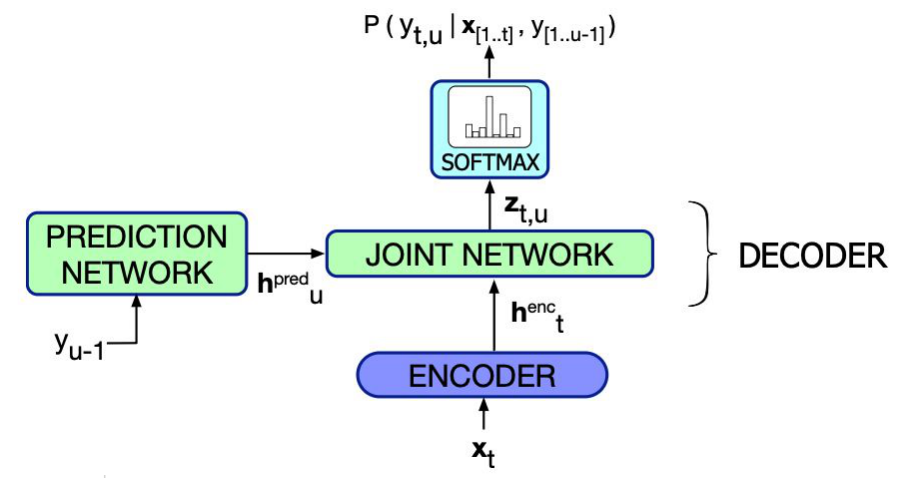
\includegraphics[width=\textwidth,height=0.72\textheight,keepaspectratio]{assets/New-Lecture-STT/cs224s_lec10_slide_47.png}
\end{frame}
